\section{Konzeption}
\label{sec_konzeption}

\subsection{Architekturbeschreibung - Serviceworker}
\label{subsec_architekturbeschreibung}

Die Anwendung beruht auf dem Client-Server-Prinzip. Dabei stellt der Client lediglich die Oberfläche zur Interaktion mit dem Anwender dar. Außer der notwendigen UI Logik ist die gesamte Geschäftslogik auf einen dedizierten (Business-)Server ausgelagert. Dieser stellt ebenfalls die Datenbank bereit. Mittels AJAX und REST werden dynamische Daten vom Client beim Server angefragt.

\begin{figure}[htp] \centering{
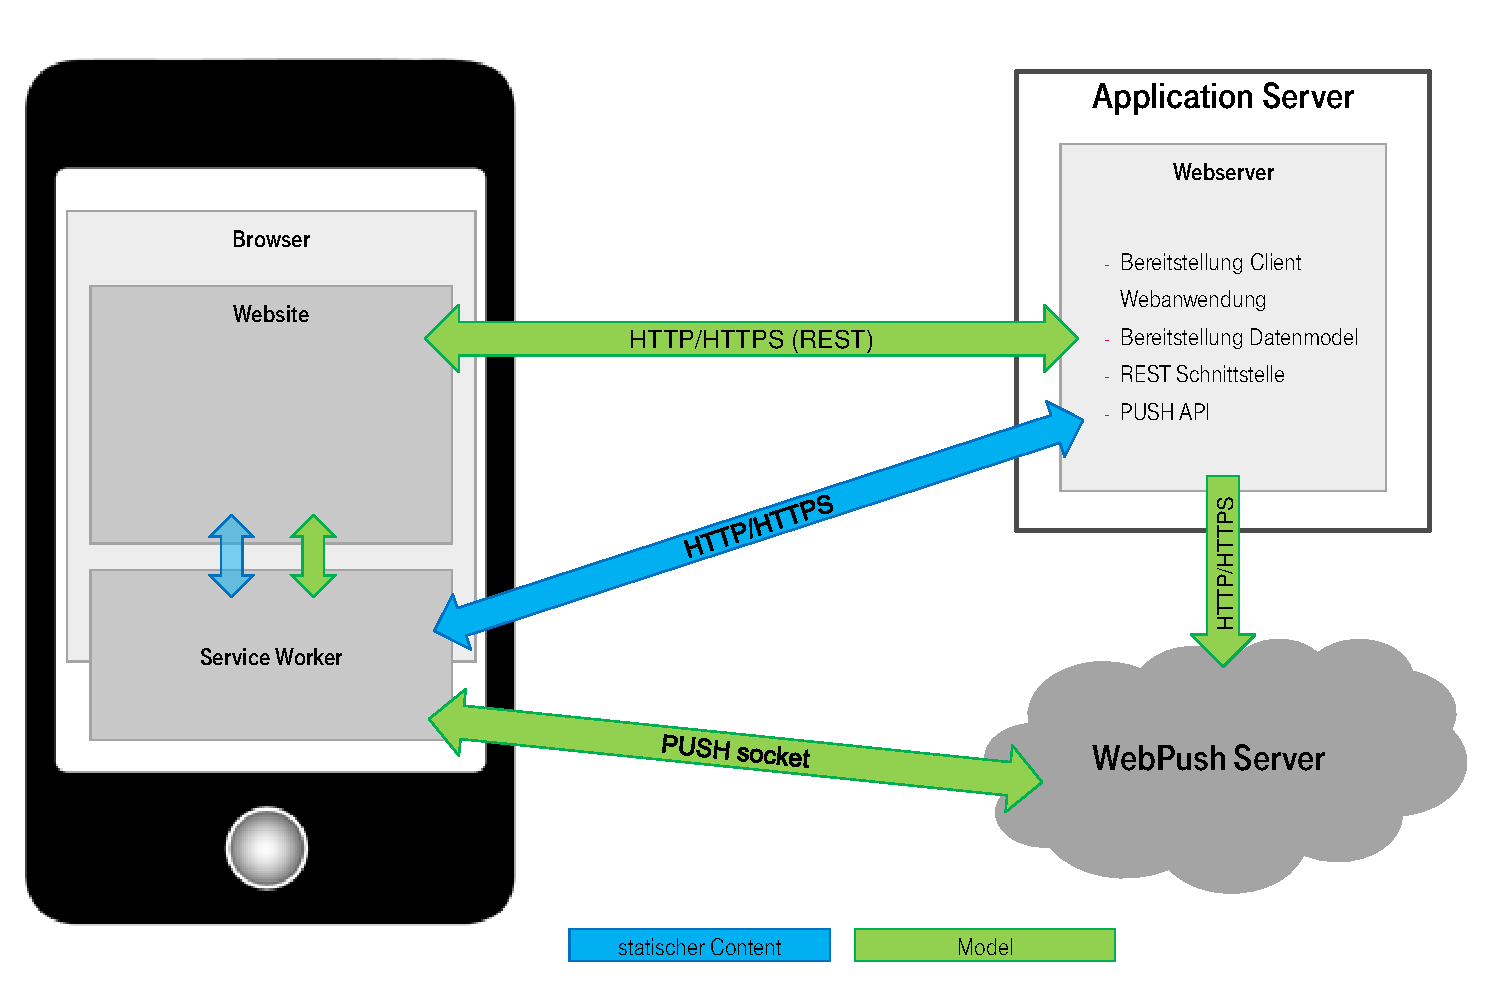
\includegraphics[width=0.9\textwidth]{images/architektur_serviceworker.pdf}}
\caption{Archtikturbeschreibung - Umsetzung mit Serviceworker}
\label{image_architektur-serviceworker-push}
\end{figure} 

\subsubsection{Push API}

\begin{figure}[htp] \centering{
\centering
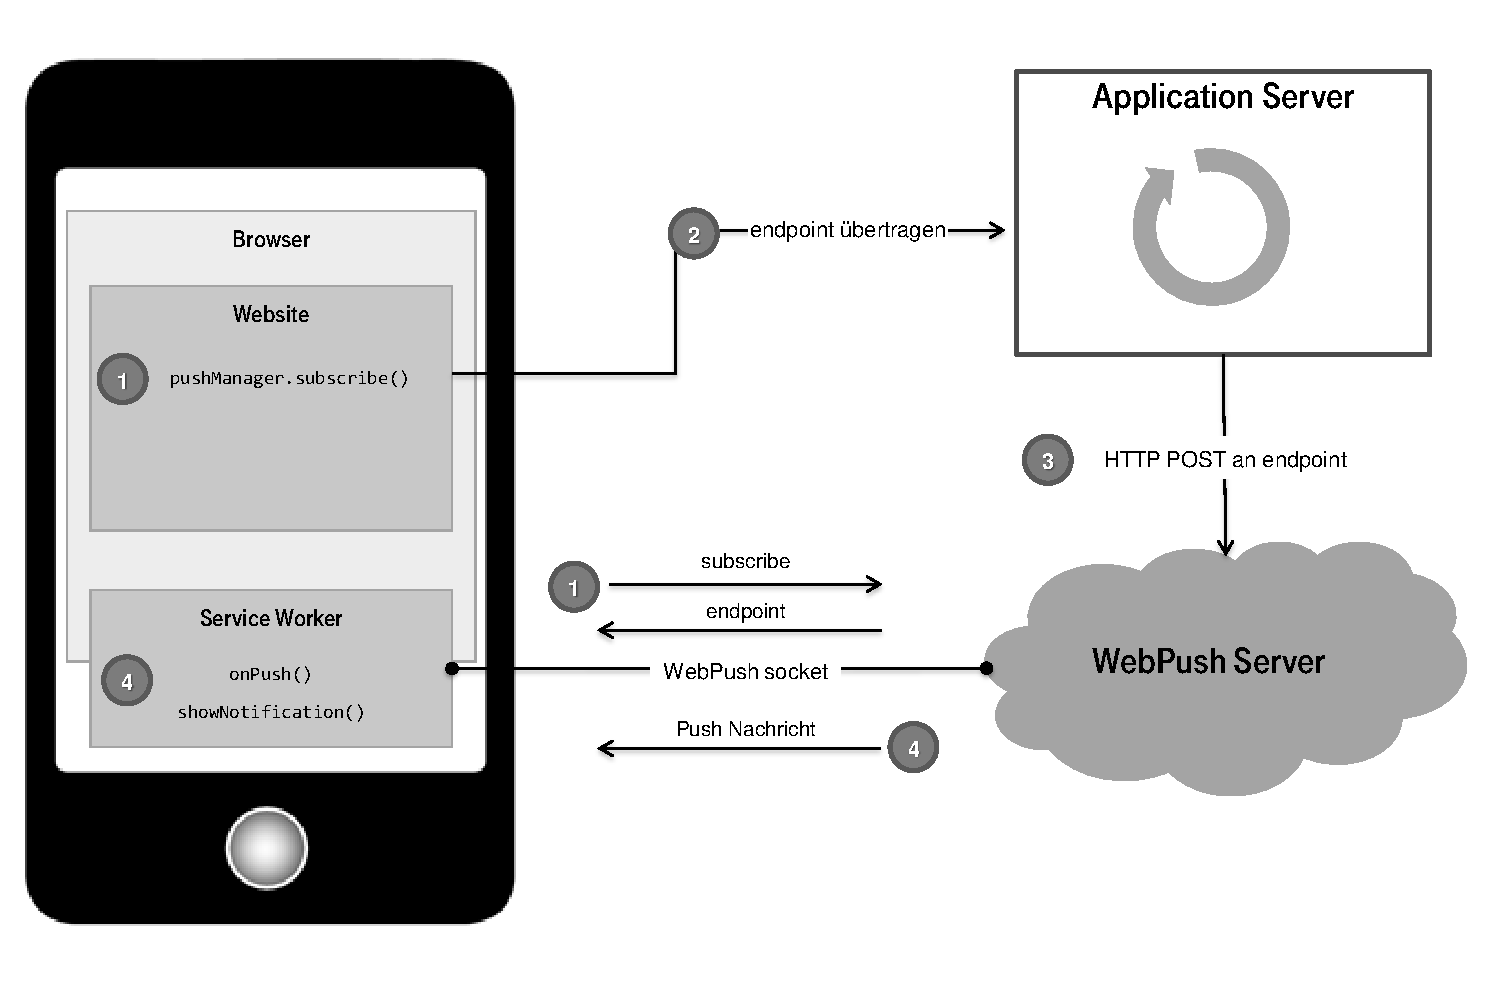
\includegraphics[width=0.9\textwidth]{images/architektur_serviceworker_push.pdf}}
\caption{Push mittels Serviceworker (in Anlehnung an MozillaWiki \cite{MOZ_WIKI})}
\quelle\url{https://wiki.mozilla.org/File:PushNotificationsHighLevel.png}
\label{image_architektur-serviceworker-push}
\end{figure}  

... Beschreibung (mit Schema) der Softwarearchitektur ...

\newpage
\subsection{Architekturbeschreibung - nativer Android Dienst}

\begin{figure}[htp] \centering{
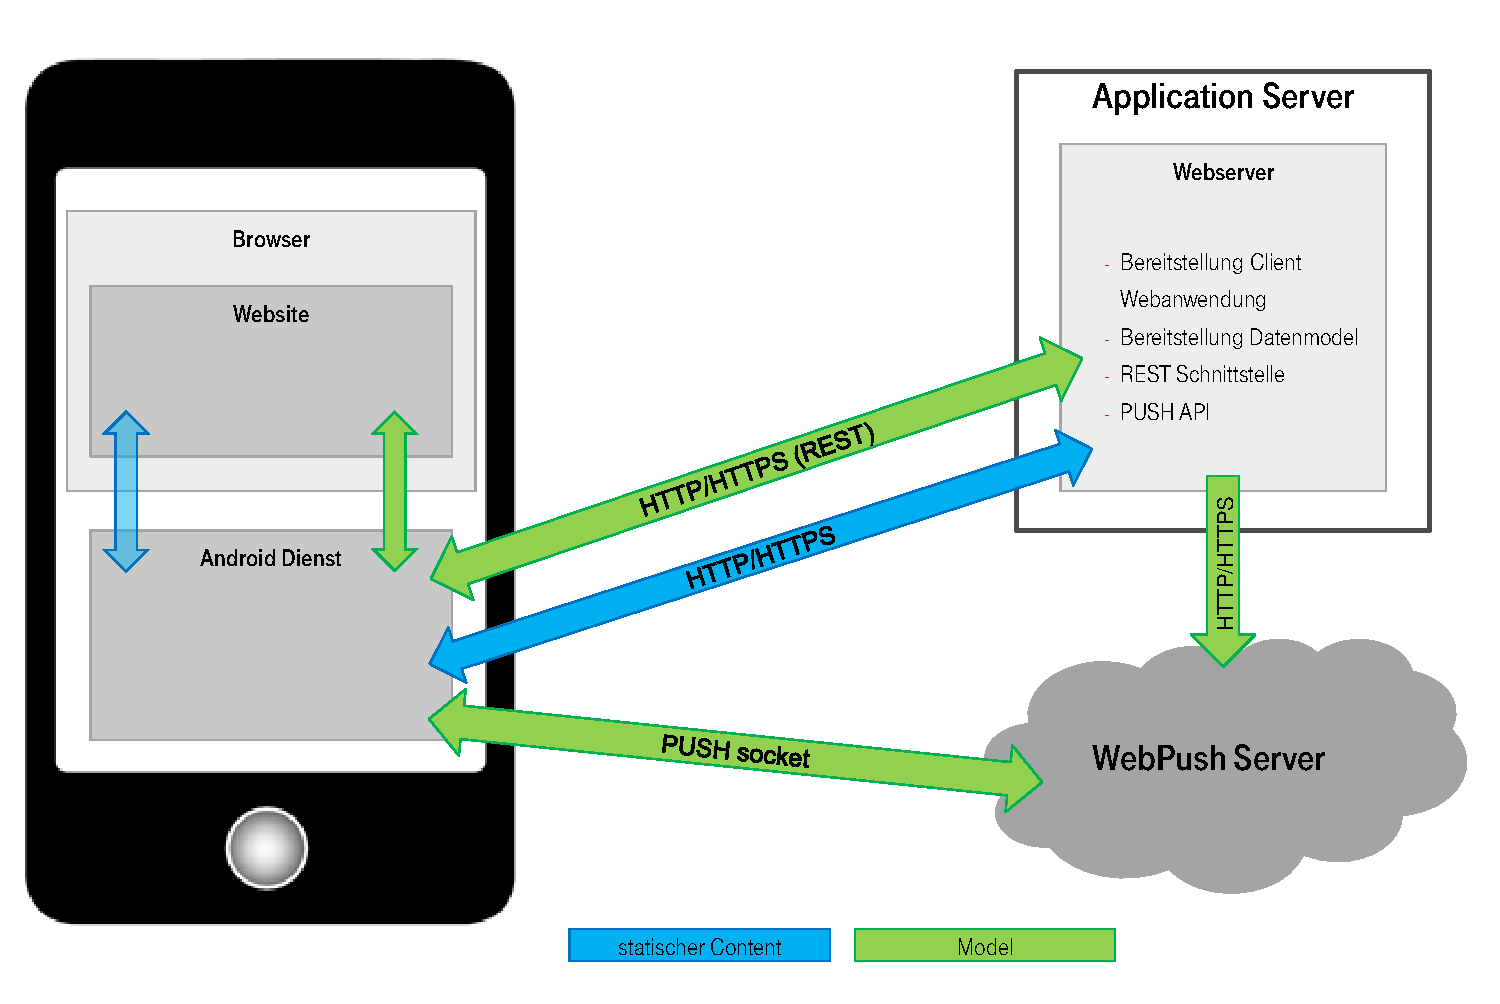
\includegraphics[width=0.9\textwidth]{images/architektur_android.pdf}}
\caption{Architektur - Umsetzung mit nativem Android Dienst }
\label{image_architektur-android-push}
\end{figure}  

... Beschreibung (mit Schema) der Softwarearchitektur ...

\subsection{Push}

\begin{figure}[htp] \centering{
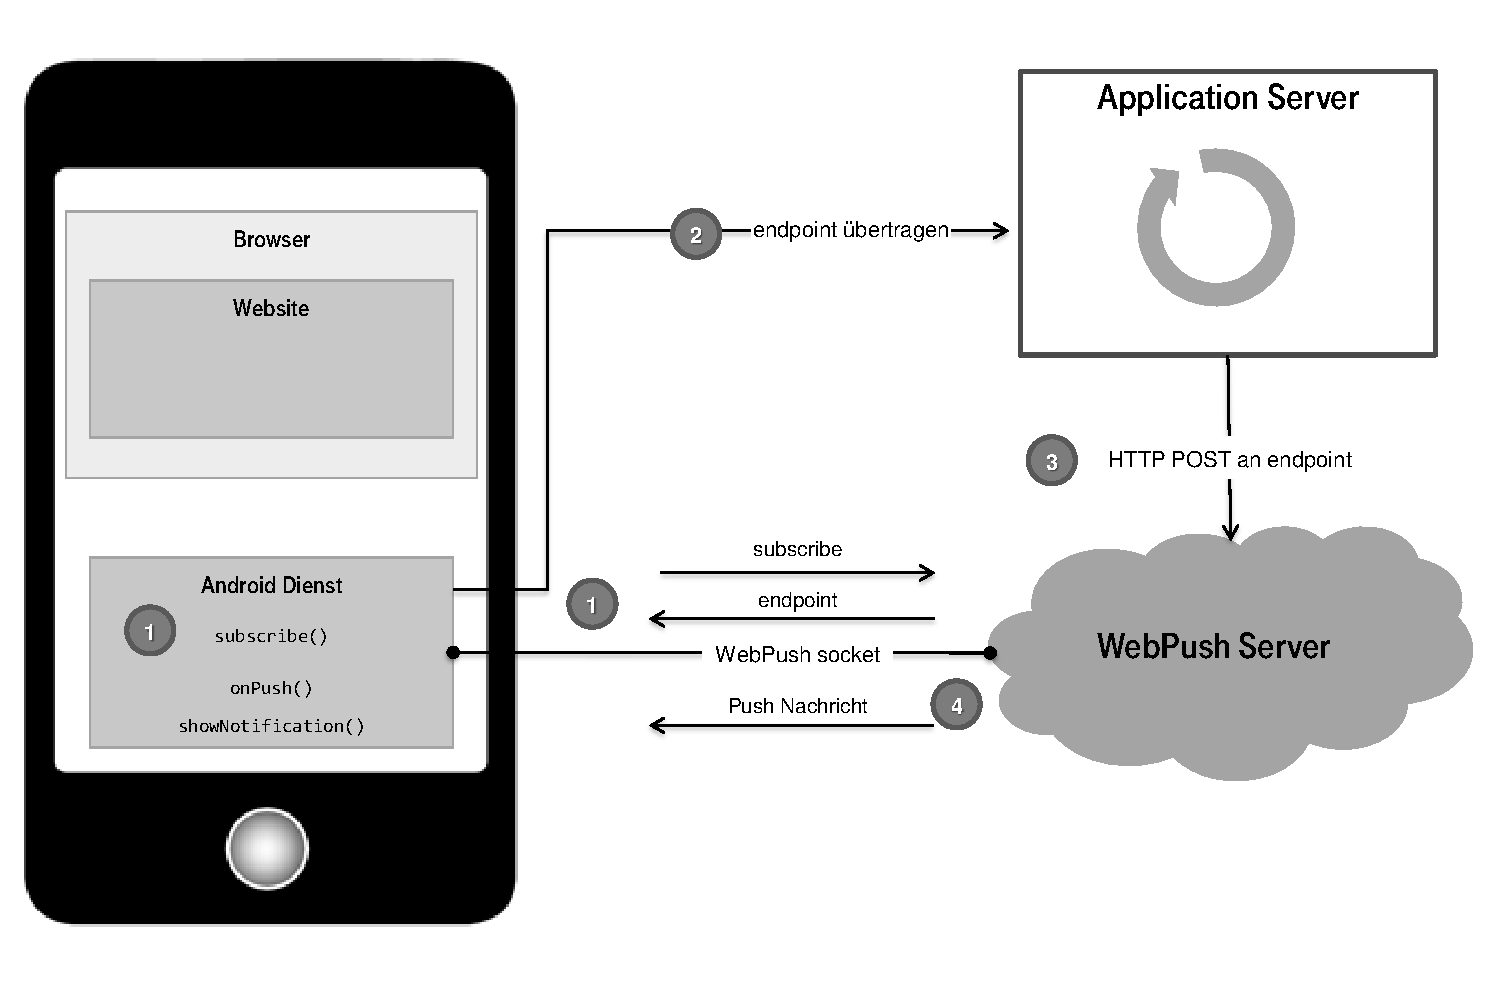
\includegraphics[width=0.9\textwidth]{images/architektur_android_push.pdf}}
\caption{Push mittels nativem Android Dienst (in Anlehnung an MozillaWiki \cite{MOZ_WIKI})}
\quelle\url{https://wiki.mozilla.org/File:PushNotificationsHighLevel.png}
\label{image_architektur-android-push}
\end{figure}  

\subsection{Datenmodell}
\label{subsec_datenmodell}



\subsection{Serverkomponente}
\label{subsec_serverkomponente}

\subsubsection{REST Schnittstelle}

\begin{table}[h]
\centering
\begin{tabular}{l | c | l }
    \textbf{Route} & \textbf{HTTP-Methode} & \textbf{Beschreibung} \\
    \hline\hline
    /api/signup & POST & Registriert einen neuen Benutzer \\
    /api/authenticate & POST & Authentifiziert einen Benutzer \\
    \hline
    /api/tasks & GET & Gibt alle Aufgaben zurück \\
    /api/tasks & POST & Legt eine neue Aufgabe an \\
    /api/tasks/:taskId & GET & Gibt eine einzelne Aufgabe zurück \\
    /api/tasks/:taskId & PUT & Aktualisiert eine einzelne Aufgabe \\
    /api/tasks/:taskId & DELETE & Löscht eine einzelne Aufgabe \\
\end{tabular}
\caption{Übersicht API Routen}
\label{tbl_api-routes}
\end{table}

\subsection{Benutzeroberfläche}

... Mockup ... \\
... Beschreibung des UI ...\\

Um das \glqq{}Look and Feel\grqq{} einer nativen App zu erreichen wird das UI-Framework \textbf{nativeDroid2} verwendet. \\

\subsection{Serviceworker}


\subsection{nativer Android Dienst}